\documentclass[a4paper,12pt]{article}
\usepackage[spanish]{babel}
\hyphenation{co-rres-pon-dien-te}
%\usepackage[latin1]{inputenc}
\usepackage[utf8]{inputenc}
\usepackage[T1]{fontenc}
\usepackage{graphicx}
\usepackage{amsmath}

\usepackage[pdftex,colorlinks=true, pdfstartview=FitH, linkcolor=blue, citecolor=blue, urlcolor=blue, pdfpagemode=UseOutlines, pdfauthor={H. Asorey}, pdftitle={Introducción a la Física - Guía 04} pdfkeywords={velocidad, aceleración, energía}]{hyperref}
\usepackage[adobe-utopia]{mathdesign}

\hoffset -1.23cm
\textwidth 16.5cm
\voffset -2.0cm
\textheight 26.0cm

\begin{document}
\begin{center}
  {\small{Universidad Industrial de Santander - Escuela de Física}}\\
  {\bf{Introducción a la Física (Asorey-Sarmiento-Pinilla)}}\\
  \vspace{0.4cm}
  Guía 04: Velocidad, Aceleración y Energía\\ 2014
\end{center}

\renewcommand{\labelenumi}{\arabic{enumi})}
\renewcommand{\labelenumii}{\arabic{enumii})}

\section*{Modalidad de Entrega}

\begin{itemize}
\item Modalidad de trabajo: grupal, en grupos con un mínimo de dos (2) y un máximo de tres (3) personas por grupo. No se admitirán trabajos individuales ni de grupos con más de tres integrantes. 
\item El trabajo será entregado utilizando el enlace dispuesta para tal fin en el blog de la materia, teniendo en cuenta lo siguiente:
\begin{itemize}
  \item la resolución de al menos uno de los ejercicios (a elección de cada grupo) deberá ser entregada en un \texttt{pdf} obtenido utilizando \LaTeX.
  \item la resolución del resto de los ejercicios puede ser realizada ``a mano'', pero todas las hojas deberán ser escaneadas
  \item se conformará un único archivo \texttt{zip} o \texttt{rar}, nombrándolo con los apellidos de los autores del trabajo en orden alfabético, separados por guiones, por ejemplo: \textit{janeway-kirk-picard.zip}, o \textit{cuadrado-gutierrez-yepes.rar}. Este archivo contendrá el \texttt{pdf} obtenido en \LaTeX, y las hojas escaneadas, y constituye el único entregable de este trabajo, que deberá ser subido al blog.
\end{itemize}
\item Para esta entrega, valen todas las indicaciones dadas para la entrega de la guía 3.
\item El cumplimiento de todas las indicaciones será tenido en cuenta.
\item {\Large{\bf{Fecha límite de entrega: Lunes 14/Julio/2014 a las 23:59:59.}}}
\end{itemize}

\section*{Cinemática}

Resuelva los siguientes ejercicios, recuerde siempre utilizar notación vectorial al resolver los ejercicios.

\begin{enumerate}
\item Una barca, que lleva una velocidad de 3\,m\,s$^{-1}$, cruza un río perpendicularmente a la dirección del agua. El río fluye a 5\,m\,s$^{-1}$ y su cauce tiene 60 metros de ancho. Hallar el ángulo y la distancia desviada. Determina la velocidad resultante, el tiempo empleado en cruzar el río y la distancia recorrida.

\item El vector de posición de un cuerpo viene dado por:
  \begin{equation}
    \vec{r} = (t^{2}+4t+1)\hat{i} + (1-5t)\hat{j}
  \end{equation}
  donde $t$ representa al tiempo y los vectores unitarios $\hat{i}=(1,0)$ y $\hat{j}=(0,1)$ son los de la base canónica de $\mathbb{R}^2$. Obtener:
  \begin{enumerate}
    \item la ecuación de la trayectoria, $\vec r(t) = \left ( x(t), y(t) \right )$;
    \item la velocidad y aceleración medias del cuerpo entre los instantes $t_{1} = 2$\,s y $t_{2} = 4$\,s;
    \item la velocidad y aceleración medias del cuerpo entre los instantes $t_{3}=4$\,s y $t_{4}=6$\,s;
  \end{enumerate}
  
\item Un avión vuela desde su campamento base al lago A una distancia $280$\,km en dirección 20$^{\mathrm{o}}$ al norte del oriente. Después de lanzar abastecimientos, vuela al lago B que esta $190$\,km y 30$^{\mathrm{o}}$ al oeste del norte del lago A. Entonces:
  \begin{enumerate}
    \item determine gráficamente la distancia;
    \item determine analíticamente el desplazamiento;
    \item determine gráfica y analíticamente la posición del lago B respecto al campamento base.
  \end{enumerate}

\item Una bola de golf es golpeada desde un \textit{tee} en el borde de un risco. Se conoce la evolución en el tiempo $t$ de las coordenadas de los vectores posición de la pelota, que siguen las siguientes expresiones:
  \begin{eqnarray}
    x(t) &=& 18t \nonumber \\
    y(t) &=& t - 49t^{2}. \nonumber\\
  \end{eqnarray}

Entonces:

  \begin{enumerate}
    \item escriba una expresión vectorial para la posición de la bola como función del tiempo, utilizando para ello los vectores unitarios $\hat{i}$ y $\hat{j}$;
    \item calcule el desplazamiento entre $t=1$\,s y $t=5$\,s;
    \item calcule la velocidad media en mismo intervalo de tiempo; 
    \item calcule la aceleración en el mismo intervalo tiempo;
  \end{enumerate}

\item Un cuerpo se mueve con rapidez inicial de $|\vec v|=3$\,m\,s$^{-1}$, y con una aceleración constante $|\vec a|=4$\,m\,s$^{-2}$. En este caso, se sabe que el vector aceleración es paralelo al vector velocidad, y ambos tienen el mismo sentido. ¿Cuál es la rapidez del cuerpo y la distancia recorrida luego de transcurrido un tiempo de $7$\,s? 
\item Resuelva ahora el problema anterior, sólo que suponiendo que la aceleración es paralela a la velocidad, pero tienen sentidos opuestos.
\item Escriba para los dos problemas anteriores, la expresión del desplazamiento como función del tiempo.

\item Un auto parte del reposo con una aceleración de $|\vec a|=1$\,m\,s$^{-2}$, la cuál se mantiene constante durante $1$\,s. Transcurrido ese tiempo, se apaga el motor y el auto desacelera, debido a la fricción, durante $10$\,s con una desaceleración promedio $|\vec a|=-5$\,cm\,s$^{-2}$. Entonces se aplican los frenos y el auto se detiene luego de otros $5$\,s adicionales. Calcular la distancia total recorrida por el auto. Hacer los gráficos de $x(t)$, $|\vec v(t)|$ y $|\vec a(t)|$ como función del tiempo $t$.
\end{enumerate}

\section*{Energía}

\begin{enumerate}
  \setcounter{enumi}{8}

\item {\bf{Energía potencial gravitatoria}}

\begin{enumerate}
\item La energía potencial gravitatoria entre dos cuerpos de masas $m_1$ y $m_2$
separados por una distancia $r$ está dada por: 
\[
E_g = -\frac{G m_1 m_2}{r}.
\]
De esta forma, la energía potencial gravitatoria de un cuerpo de masa $m$ sobre
la superficie de un planeta de masa $M$ y radio $R$ es: 
\[
E_g = -\frac{G M m}{R}.
\]
Verifique que al elevar ese cuerpo a una altura $h$ sobre la superficie del
planeta, la variación de la energía potencial gravitatoria es: 
\[
\Delta E_g = - G M m \left ( \frac{1}{R+h} - \frac{1}{R} \right ).
\]
\item Calcule la variación de energía potencial gravitatoria para un astronauta de masa $m=70$\,kg, que originalmente se encontraba sobre la superficie terrestre ($h=0$) y luego a una altura de $h=370$\,km, correspondiente a la órbita media de la estación espacial internacional (ISS). Luego, compare ese valor con el que hubiera obtenido utilizando la expresión aproximada $\Delta E_g = m g h$, donde $g$ corresponde al valor de la aceleración de la gravedad sobre la superficie terrestre, $g=9.81$\,m\,s$^{-2}$ . ¿Cuál es la diferencia porcentual obtenida al utilizar la fórmula aproximada?
\end{enumerate} 

\item {\bf{Pesos}}.

A partir de la definición de la aceleración de la gravedad $g\equiv |\vec g|$ sobre la superficie de un cuerpo de masa $M$ y radio $R$, 
\[ g=\frac{GM}{R^2}, \]
\begin{enumerate}
  \item calcule el valor de $g$ y determine cuál es el peso de un cuerpo de masa $m=70$\,kg en la Tierra, el Sol, Júpiter, Marte y la Luna (use los datos para $M$ y $R$ reproducidos al final de esta guía).
  \item Repita las cuentas realizadas en clase y, utilizando la segunda Ley de Newton $\vec F=m \vec a$ verifique que el peso de un cuerpo de masa $m$ como función de la altura $h$ sobre la superficie del cuerpo de masa $M$ y radio $R$ es: 
    
    \[ |\vec F_p(h)| = m \left ( \frac{G M}{(R + h)^2} \right ) = m g(h). \]

    Observe que a partir de esta expresión, el módulo de la fuerza peso depende de la altura sobre la superficie del cuerpo de masa $M$, y se puede expresar en general como $F_p(h) = m g(h)$. En este caso, la dirección de la fuerza peso es radial, y el sentido hacia el centro del objeto de masa $M$.
  \item Obtenga a que altura $h_2$ sobre la superficie el peso de un cuerpo vale la mitad respecto a su peso sobre la superficie ($h=0$).
  \end{enumerate}

\item {\bf{Rebotes}}.

Una pelota de goma de masa $m=2.0$\,kg es lanzada hacia arriba en forma vertical. La rapidez inicial es de $v=5$\,m s$^{-1}$.
\begin{enumerate}
\item Calcule la altura máxima que alcanza la pelota en su trayectoria; 
\item suponiendo que no hay pérdidas de energía debidas al rozamiento, calcule la rapidez al momento del impacto y la altura alcanzada luego del rebote. 
\item Suponga que, a diferencia del punto anterior, como consecuencia del rebote un $20\%$ de la energía mecánica se transforma en calor y sonido. Calcule la altura que alcanzará la pelota luego de tres choques contra el piso.
\end{enumerate}

\item{\bf{Resortes}}

La energía potencial elástica está dada por:
\[E_e = \frac{1}{2} k (\Delta x)^2 \]
donde $k$ es la constante elástica del resorte y $\Delta x$ representa a la variación de la longitud del resorte en condiciones de compresión o expansión. Imagine entonces que usted debe diseñar el sistema de protección de resortes de un ascensor en un edificio ($h=50.0$\,m), y que los mismos pueden comprimirse un máximo de $0.5$\,m. Sabiendo que la masa del ascensor y su carga es de $m=600$\,kg,

\begin{enumerate}
\item calcule la constante $k$ del resorte;
\item si el ascensor tiene un freno de seguridad capaz de transformar el $20\%$ de la energía cinética, calcule el $k$ del resorte necesario en este caso;
\item Rehaga los cálculos anteriores pero suponiendo que en lugar de un único gran resorte se disponen cuatro resortes más pequeños.
\end{enumerate}

\item {\bf{Velocidad de escape}}

Se define como {\emph{velocidad de escape}} a aquella velocidad $v_c$ para la cual un cuerpo de masa $m$ (cuerpo A) puede escapar de la atracción gravitatoria de otro cuerpo (cuerpo B).

Imaginemos que el cuerpo B es un planeta de radio $R$ y masa $M$, y colocamos al cuerpo A sobre su superficie. Entonces,
 
\begin{enumerate}
\item Obtenga una expresión para el cálculo de la velocidad de escape, y muestre que la misma es una propiedad inherente del planeta.
\item Grafique la dependencia de la velocidad de escape como función:
\begin{itemize}
\item del radio $R$ del planeta.
\item de la masa $M$ del planeta.
\end{itemize}
\item Calcule el valor de la velocidad de escape sobre la superficie de 
\begin{enumerate}
\item el planeta Tierra,
\item la Luna,
\item el planeta Marte,
\item el Sol.
\end{enumerate}
\item Luego, verifique que la expresión para el $R$ de un objeto de masa $M$ para que la velocidad de escape sobre su superficie sea igual a la velocidad de la luz $c$, 
  \[ R_c = \frac{2GM}{c^2}.\]  
  Con esta expresión, calcule el valor del radio crítico $R_c$ para la Tierra, el Sol, y un objeto con masa $M=10 M_{\mathrm{Sol}}$.

\end{enumerate}

\item {\bf{Impacto}}.

La extinción de los dinosaurios al final del período Jurásico es atribuida al impacto de un cometa o meteorito de dimensiones considerables. Imagine entonces que un cometa esférico de radio $r=5$\,km y densidad media $d=5$\,g\,cm$^{-3}$ se acerca a la Tierra desde el infinito. Entonces,

\begin{enumerate}
\item Calcule la masa $m_c$ del cometa.
\item Calcule la energía cinética y la velocidad al momento del impacto.
\item Exprese la energía liberada en el impacto en megatones, teniendo en cuenta que $1$\,Mton $= 4.184 \times 10^{15}$\,J.
\item Si debido a la interacción atmosférica el satélite se divide en dos partes de masas $m_1=0.7 m_c$ y $m_2=0.3 m_c$. Calcule la energía cinética y la velocidad de cada parte al momento del impacto. ¿Dependerá el resultado de la altura a la cual el cometa se parta? Justifique.
\end{enumerate}

\item {\bf{El Principito}}

El Principito ($m=40$\,kg) vive en un planeta pequeño, el asteroide B612. Supongamos que posee un radio $R = 1$\,km con una densidad igual a la de la Tierra ($d = 5.5$\,g\,cm$^{-3}$). Calcule 
\begin{enumerate}
\item el valor de $g$ y el peso del Principito en B612;
\item si en la Tierra el Principito logra subir a una silla de $h=0.5$\,m de un salto, a que altura llegará con el mismo salto sobre la superficie de B612. 
\item la velocidad máxima a la cual el Principito puede caminar sin riesgo de abandonar el planeta para siempre
\end{enumerate}
\end{enumerate}
\centering 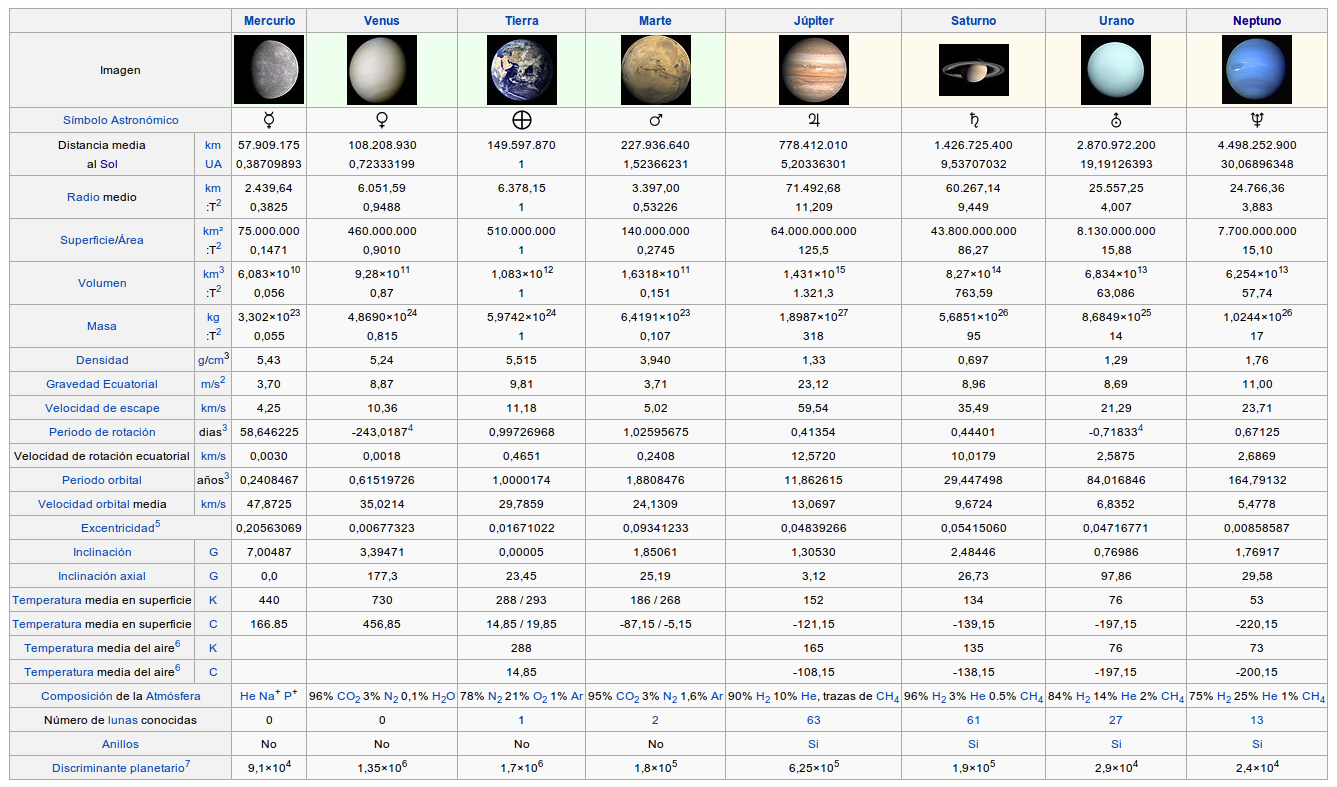
\includegraphics[height=11.6cm,angle=90]{planetas.png}

\end{document}
%%%%
